%%%
%  File: chapter3.tex
%  Project: rp-doc
%  Author: Javier Reyes
%  Created on: 26.08.2018
%  
%  Last modified: 08.09.2018
%  Modified by: Javier Reyes (javier.reyes.g@gmail.com)
%  
%  MIT License
%  
%  Copyright (c) 2018 Javier Reyes
%  
%  Permission is hereby granted, free of charge, to any person obtaining a copy of
%  this software and associated documentation files (the "Software"), to deal in
%  the Software without restriction, including without limitation the rights to
%  use, copy, modify, merge, publish, distribute, sublicense, and/or sell copies
%  of the Software, and to permit persons to whom the Software is furnished to do
%  so, subject to the following conditions:
%  
%  The above copyright notice and this permission notice shall be included in all
%  copies or substantial portions of the Software.
%  
%  THE SOFTWARE IS PROVIDED "AS IS", WITHOUT WARRANTY OF ANY KIND, EXPRESS OR
%  IMPLIED, INCLUDING BUT NOT LIMITED TO THE WARRANTIES OF MERCHANTABILITY,
%  FITNESS FOR A PARTICULAR PURPOSE AND NONINFRINGEMENT. IN NO EVENT SHALL THE
%  AUTHORS OR COPYRIGHT HOLDERS BE LIABLE FOR ANY CLAIM, DAMAGES OR OTHER
%  LIABILITY, WHETHER IN AN ACTION OF CONTRACT, TORT OR OTHERWISE, ARISING FROM,
%  OUT OF OR IN CONNECTION WITH THE SOFTWARE OR THE USE OR OTHER DEALINGS IN THE
%  SOFTWARE.
%%%

\chapter{Embedded Linux} \label{embedded-linux}

In order to have a usable stack implementation of Ethernet communication, it is recommended to boot
an OS in the device, considering time and complexity for a standalone driver implementation of an
Ethernet stack driver for the specific hardware configuration present in the Zynqberry.

Xilinx provides a workflow to create an embedded Linux image fitted for the ARM architecture, by
means of a provided tool (a collection of command-line programs) to configure and compile
Linux-based images focused on Xilinx hardware, using Yocto Project.

\section{Xilinx Petalinux}

Xilinx Petalinux is an Embedded Linux System Development Kit for Xilinx FPGA-based System-on-Chip
devices\cite{UG1144}. It is based on Yocto Project SDK's for the Xilinx hardware architectures
(Zynq, Zynq UltraScale+, MicroBlaze full and lite).

The specific workflow for the tool can be different depending on the hardware platform and the
desired application(s). As a reference, an overview flow is shown in the table
\ref{table:design-flow-overview}.

\begin{table}[ht]
	\centering
	\footnotesize
	\begin{tabular} {| l | l |}
		\hline
		\textbf{Design Flow Step} & \textbf{Tool / Workflow} \\ [0.25cm]
		\arrayrulecolor[HTML]{B20738} 
		\hline \arrayrulecolor[HTML]{000000}
		Hardware Platform Creation & Vivado \\
		\hline
		Create Petalinux Project & petalinux-create -t Project \\
		\hline
		Initialize Petalinux Project & petalinux-config --get-hw-description \\
		\hline
		Configure System-Level Options & petalinux-config \\
		\hline
		Create User Components & petalinux-create -t COMPONENT \\
		\hline
		Configure the Linux Kernel & petalinux-config -c kernel \\
		\hline
		Configure the Root Filesystem & petalinux-config -c rootfs \\
		\hline
		Build the System & petalinux-build \\
		\hline
		Deploy the System & petalinux-package \\
		\hline
		Test the System & petalinux-boot \\
		\hline
	\end{tabular}
	\caption{Design Flow Overview, from \cite{UG1156}}\label{table:design-flow-overview}.
\end{table}

The Zynqberry board has a specific hasrdware configuration that requires a unique flow for building
an embedded Linux image. Therefore, most of the standard flow cannot be applied directly. The
followed procedure for this project is detailed in the Appendix \ref{appen1}.

\section{Yocto Project}

The core of the Petalinux tool is the Yocto SDK, an open-source community project that allows to
create custom Linux-based systems for embedded products, independent of the hardware architecture.
It consists of a flexible toolset and a development environment, allowing software customizations
and build interchange for multiple hardware platforms as well as maintainable and scaled software
stack.

\begin{figure}[htp]
	\centering
	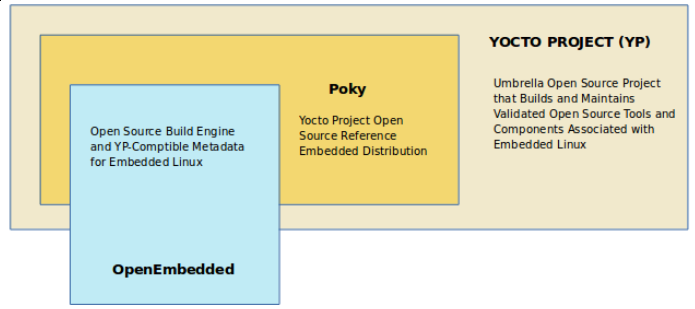
\includegraphics[width=0.7\textwidth]{yocto-project-block.png}
	\caption{Yocto Project structure, from \cite{yocto-manual}.} \label{fig:yocto-project-block}
\end{figure}

\subsection{Layer Model}

The Yocto development model defines a layered structure, as repositories that contain configurations
and instructions for the OpenEmbedded build system to know what and how to build the system. The
layer model allows to logically separate information in the build. If a layer needs to specify in
another layer, a recipe defined in a BitBake append (\texttt{.bbapend}) file.

The common recommended workflow is based on a reference distribution (\textit{Poky}), which contains
the OpenEmbedded build system and the set of metadata necessary to start building the IoT
distribution.

\begin{figure}[htp]
	\centering
	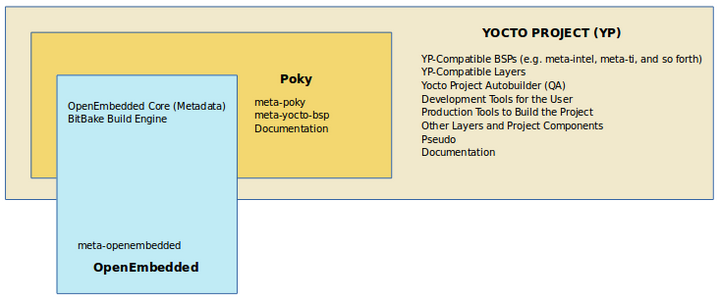
\includegraphics[width=0.7\textwidth]{yocto-poky.png}
	\caption{Content of a typical Poky repository, from \cite{yocto-manual}.} \label{fig:yocto-poky}
\end{figure}

\subsection{OpenEmbedded Build System Workflow}

The expected workflow can be represented in figure \ref{fig:yocto-workflow}, where the different
actors are identified as well as the expected outputs. This process can be shortly summarized as
follows:

\begin{enumerate}
	\item Specify architecture, policies, patches and configurations.
	\item Fetch and download of source codes.
	\item Sources extraction, patches applying and configuring and compiling the software.
	\item Software installing.
	\item Quality assurance and sanity checks for the entire build process.
	\item Binary package feed is used to create the final root file image.
	\item The build system generates the file system image and the Extensible SDK in parallel.
\end{enumerate}

\begin{figure}[htp]
	\centering
	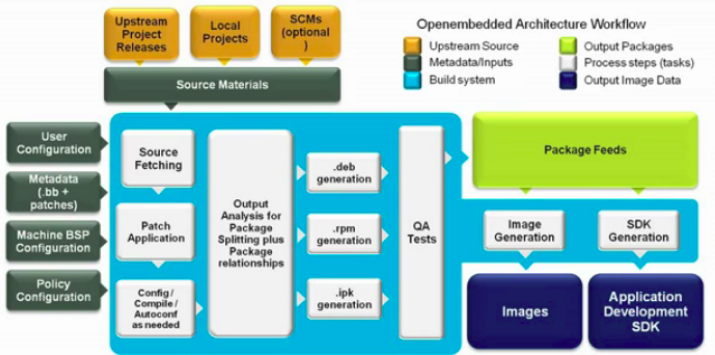
\includegraphics[width=0.7\textwidth]{yocto-workflow.png}
	\caption{Default Build System workflow, from \cite{yocto-manual}.} \label{fig:yocto-workflow}
\end{figure}

\section{Boot Up Sequence}

The embedded Linux built for this project requires a non-standard boot up flow, as the Znyq7 XC7Z010
chip has not enough MIO pins for the hardware that would allow the first boot read from an SD card
reader. Therefore, a custom boot up sequence was needed. Additional, the board model was discovered
to be a non-standar model (the typical model for the TE0726 includes 512MB of DDR3 RAM memory,
whereas the model used is a 128 MB version), which created difficulties to find suitable
documentation for this specific hardware configuration.

The process is detailed in the Appendix \ref{appen1}. As a general rule, the hardware definition for
the PS needs to be done via a reference design project provided by the manufacturer using prepared
scripts, as opposed to the usual Xilinx workflow where a user-defined board should provide a TCL
preset file with the necessary configuration values for the IP Core.

Once the hardware has been correctly defined and exported, the Linux image build process needs to
consider also the special configuration for the 128 MB memory capacity, which proved to be still a
process with several iterations needed as the documentation and support is limited in terms of the
manufacturer capabilities. The configuration also needs to define the boot process to the specific
Zynq hardware configuration.

\subsection{Linux Boot}

\begin{figure}[htp]
	\centering
	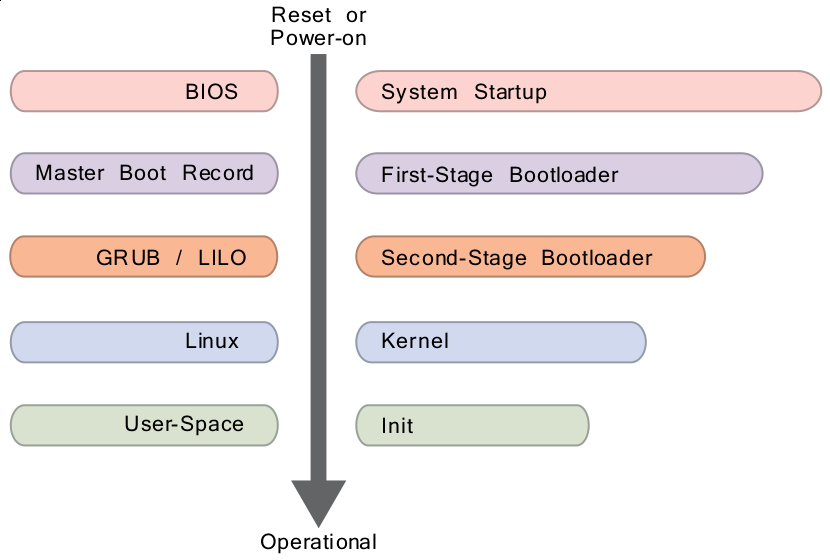
\includegraphics[width=0.6\textwidth]{linux-boot.png}
	\caption{Stages of a Linux boot process, from \cite{Crokett2014}.} \label{fig:linux-boot}
\end{figure}

\subsection{Zynq Boot}

The specific process for the Zynqbery 726 board used in the project needs special considerations
that are hardware-related. In general, the workflow provided by Xilinx needs to be slighltly
modified, and use the board manufacturer documentation and scipts. This is due to the fact that the
board uses specific hardware, and the documentation provided does not match, as the Zynqberry
hardware cannot direct boot from the SD card reader. Once the image (and other relevant binary
files) have been correctly build, special care needs to be taken to generate the BOOT.BIN file for
the stage-0 boot process. More detailed instructions are provided in Appendix \ref{appen1}.

\begin{enumerate}
	\item Power up of the board starts.
	\item The BOOT.BIN binary is read from flash memory through QSPI and run.
	\item From this binary, the First Stage Boot Loader is then loaded, which will configure the PS
	and PL, and then locate and load the u-boot into DDR memory.
	\item U-boot will initialize the hardware, and then unpack and load the linux kernel.
	\item Once the kernel is loaded into the high memory, specific hardware setup is run.
	\item When kernel is ready, the first user-space application (\textit{init}) can start.
\end{enumerate}

\section{Xilinx Linux embedded OS}

In order to have a runnable Linux OS, the building process in Petalinux SDK needs to configure the
kernel and the RootFS, as the default configuration expects a standard boot from SD card for the
entire sequence. Also, a memory offset parameter needs to be adjusted for the 128MB RAM memory size.

\begin{figure}[htp]
	\centering
	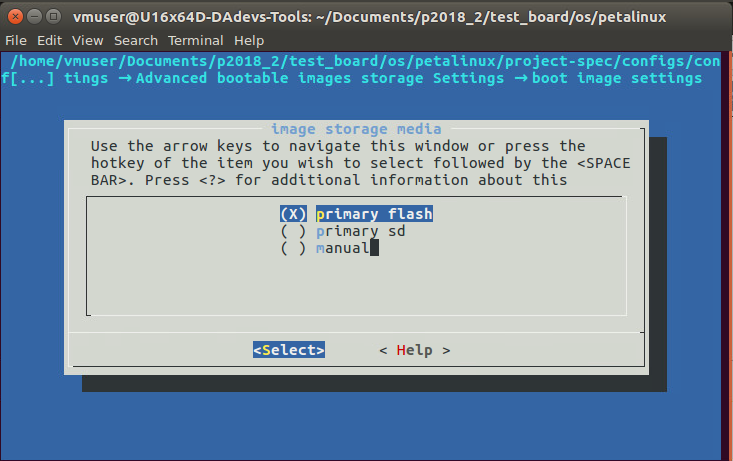
\includegraphics[width=0.7\textwidth]{boot-img-source-config.png}
	\caption{Configuration of BOOT image source in Petralinux kernel config.}
	\label{fig:boot-img-source-config}
\end{figure}

\begin{figure}[htp]
	\centering
	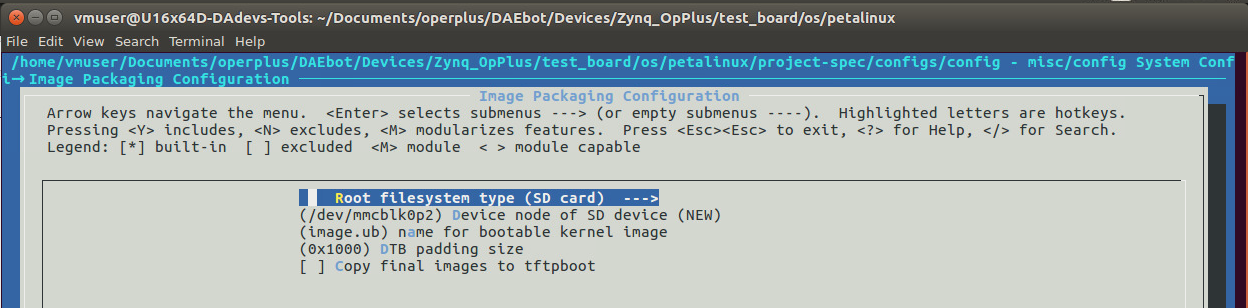
\includegraphics[width=0.7\textwidth]{boot-img-rootfs.png}
	\caption{Configuration of rootfs type in Petralinux kernel config.}
	\label{fig:boot-img-rootfs}
\end{figure}

\begin{figure}[htp]
	\centering
	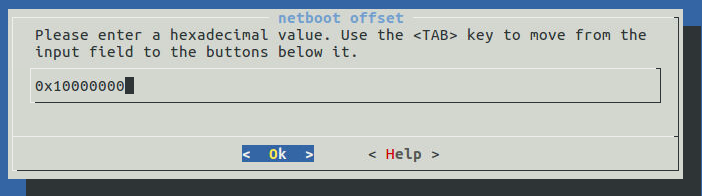
\includegraphics[width=0.7\textwidth]{boot-img-offset.png}
	\caption{Configuration of memory offset Petralinux kernel config.}
	\label{fig:boot-img-source-offset}
\end{figure}

Once the kernel has been configured, the build can be started. This process is high CPU consuming,
and depending on the host, can take several minutes. After succesful completion, the built image
will be located in \texttt{petalinuxFolder/images/linux}. For this project, only the OS image
(\texttt{image.ub}) and the FSBL application (\texttt{u-boot.elf}) are relevant.

With help of the Xilinx XDK utility, the \texttt{BOOT.BIN} file can be created, by means of the
FPGA bitstream and the FSBL application. There is also a TCL script from the board manufacturer that
performs the binary creation and the programming to the FLASH chip memory. It should be noted that
in case of a specific non-default functionality expected from the FSBL, the compiled
\texttt{u-boot.elf} will not work for flash programming, as Vivado uses a specific setting that
cannot be fullfiled with the tools. Manufacturer provides a precompiled default version of FSBL for
programming, otherwise a special project with hardware tricks need to be created for the FSBL
generation only.

The SD card for the OS should be formatted as follows:

\begin{itemize}
	\item First partition - ~ 512 MB - FAT32
	\item Second partition - Rest of space - EXT2 or EXT4
\end{itemize}

The OS image will be located in the first partition. The desired FileSystem will be located into the
second partition (ensuring that space is enough for it). For this project, an Ubuntu 16.04 LTS
File System is used.

With the flash programmed and the SD correctly loaded, the boot process can be started, as shown in
figure \ref{fig:boot-start}. For testing purposes, a serial console is opened through the port
that the Xilinx driver creates for the board, with Baud rate of 115200 bps and default bits of
start/stop. Once the boot has been validated, the IP address assigned to the device can be checked
(with \texttt{ifconfig}) and an ssh connection can be performed (ssh should be by default included
in the OS, otherwise it can be installed with \texttt{apt}).

\begin{figure}[htp]
	\centering
	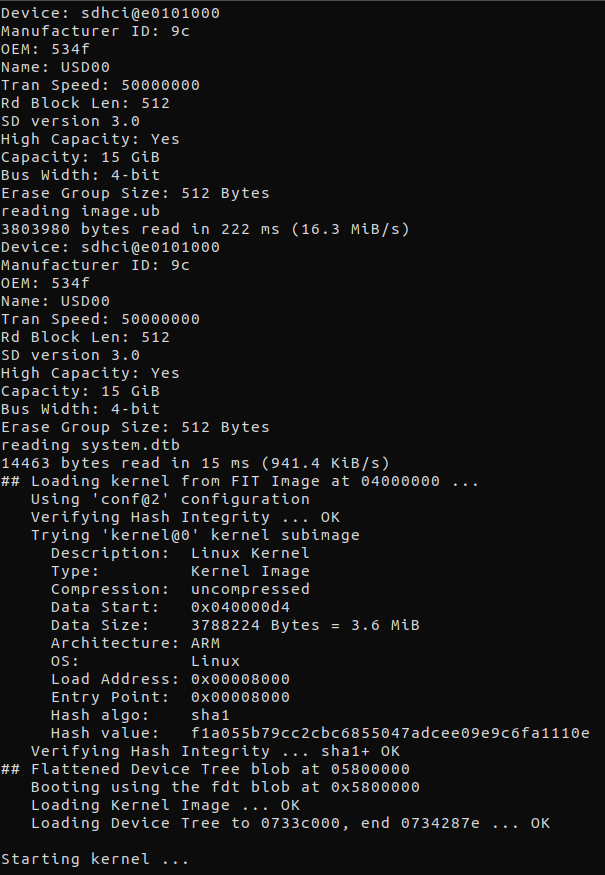
\includegraphics[width=0.7\textwidth]{boot-start.png}
	\caption{Start of the boot up process in the Zynqberry board.}
	\label{fig:boot-start}
\end{figure}

The login user has been renamed for more comprehensive usage, as shown in figure 
\ref{fig:boot-login}.

\begin{figure}[htp]
	\centering
	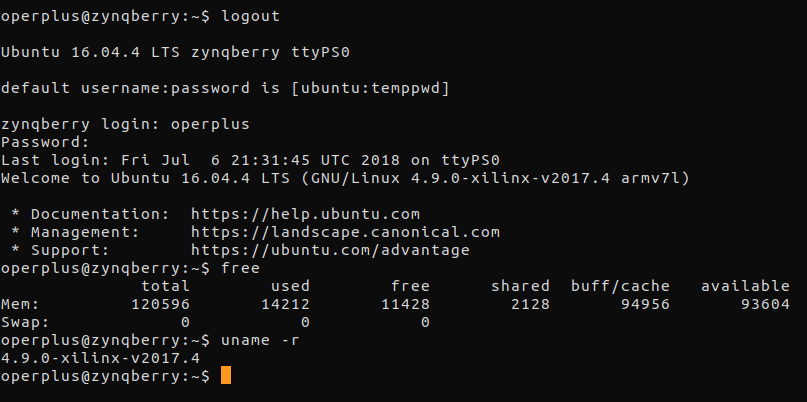
\includegraphics[width=0.7\textwidth]{boot-login.png}
	\caption{User logged into the Ubuntu 16.04.4 LTS Zynqberry.}
	\label{fig:boot-login}
\end{figure}
